\documentclass[border=8pt]{standalone}
\usepackage[T1]{fontenc}
\usepackage[utf8]{inputenc}
\usepackage{tikz}
\usetikzlibrary{arrows.meta}
\begin{document}
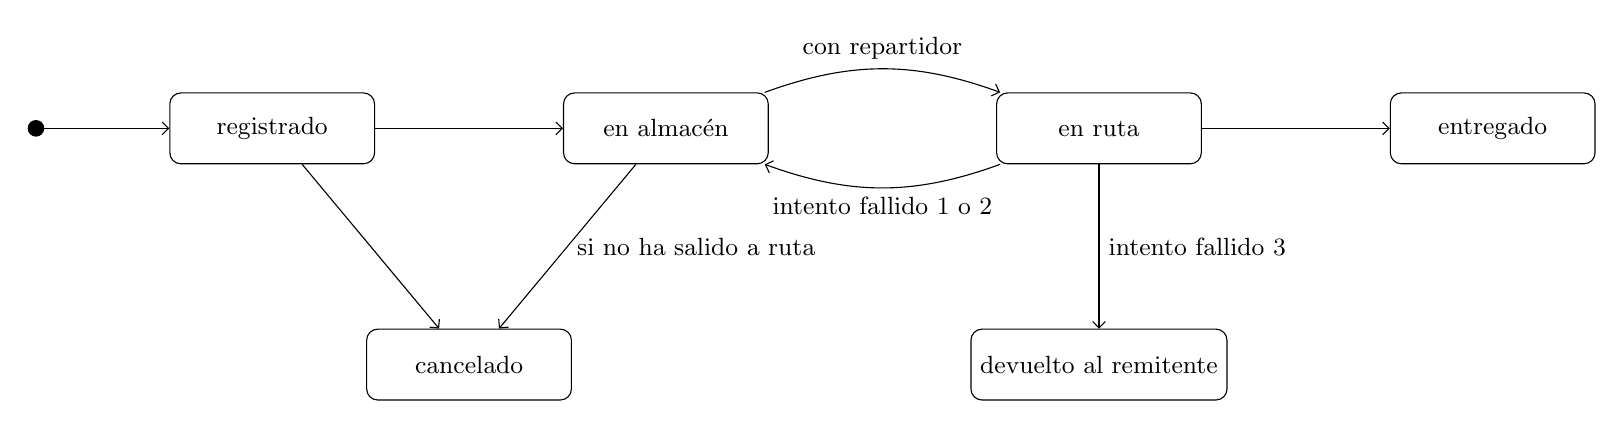
\begin{tikzpicture}[e/.style={draw,rounded corners,minimum width=2.6cm,minimum height=9mm},>=Straight Barb,font=\small]
\fill (-3,0) circle (3pt);
\node[e] (r) at (0,0) {registrado};
\node[e] (a) at (5,0) {en almacén};
\node[e] (u) at (10.5,0) {en ruta};
\node[e] (d) at (15.5,0) {entregado};
\node[e] (c) at (2.5,-3) {cancelado};
\node[e] (v) at (10.5,-3) {devuelto al remitente};
\draw[->] (-2.9,0) -- (r);
\draw[->] (r) -- (a);
\draw[->] (a) to[bend left=20] node[above]{con repartidor} (u);
\draw[->] (u) to[bend left=20] node[below]{intento fallido 1 o 2} (a);
\draw[->] (u) -- (d);
\draw[->] (u) -- node[right]{intento fallido 3} (v);
\draw[->] (r) -- (c);
\draw[->] (a) -- node[right]{si no ha salido a ruta} (c);
\end{tikzpicture}
\end{document}
